%%
%% ----------------------------------------------------------------
%% Copyright (C) 2023-2024 by Simon Pfahler <simon.pfahler at ur dot de>
%% ----------------------------------------------------------------
%%
%! TeX program = lualatex
\documentclass{scrartcl}
\usepackage[left=4cm,right=3cm,top=3cm,bottom=3cm, marginpar=3cm]{geometry}
\setlength{\parindent}{0pt}
\setlength{\parskip}{1ex}

\usepackage{cprotect}
\usepackage{tikz}
\usetikzlibrary{math}

\usepackage{xcolor}
\usepackage{soul}

\usepackage{tikz}
\usetikzlibrary{positioning, shapes, fit, arrows.meta, decorations.pathmorphing}
\pgfdeclarelayer{bg}
\pgfsetlayers{bg,main}

\usepackage{pgfplots, pgfplotstable}
\pgfplotsset{compat=1.18}

%%%% from https://tex.stackexchange.com/questions/355713/pgfplots-show-error-marker-in-legend
\pgfplotsset{error bar legend/.style={%
    /pgfplots/legend image code/.prefix code={%
      \pgfkeysgetvalue{/pgfplots/error bars/error mark}{\pgfplotserrorbarsmark}%
      \draw[%
        /pgfplots/every error bar,
        mark=\pgfplotserrorbarsmark,
        /pgfplots/error bars/error mark options,
        sharp plot,
        ##1
      ] plot coordinates {(0.3cm, -0.15cm) (0.3cm, 0.15cm)};%
    }
  }
}
%%%%

\pgfplotsset{custom area legend/.style={%
    /pgfplots/legend image code/.prefix code={%
        \fill[##1, draw=white] plot coordinates {(0cm, -0.1cm) (0.6cm,-0.1cm) (0.6cm, 0.1cm) (0cm, 0.1cm)};%
    }
  }
}

\def\w{420pt}

\usepackage{hyperref}
\hypersetup{
    pdftitle={Easy colorblind-safe typesetting: the colorblind package},
    pdfauthor={Simon Pfahler},
}
\usepackage{cleveref}

\usepackage{csquotes}
\usepackage[backend=biber, style=numeric-comp, seconds=true, sorting=none, subentry=true, doi=false, alldates=iso]{biblatex}
\renewcommand*{\entrysetpunct}{\\[5pt]}
\addbibresource{bib.bib}

\usepackage[Tol, OkabeIto, pgf]{colorblind}

\newcommand\colorblind{\textbf{colorblind} }
\newcommand\hlc[2][T-Q-PH4]{{%
    \colorlet{foo}{#1}%
    \sethlcolor{foo}\hl{#2}}%
}

\reversemarginpar
\newcommand\marg[1]{\leavevmode\marginpar{\raggedleft #1}}
\newcommand\tbs{\textbackslash}

\title{Easy colorblind-safe typesetting:\\ the \colorblind package}
\author{Simon Pfahler}
\date{\today\\Version 1.0.1}


\begin{document}

\maketitle

\begin{abstract}
    In colorblind-safe documents, the contents are presented in a way that the same information is conveyed to readers regardless of a potential color vision deficiency.
    This package provides the tools necessary for colorblind-safe typesetting in \LaTeX.
    It provides color schemes for a wide range of applications.
    The most commonly used schemes are qualitative schemes, providing easily distinguishable colors for use in graphics, but also for text coloring or highlighting.
    Additionally, diverging and sequential schemes are included which can be used for encoding quantitative information using colors.
    This package incorporates colorblind-safeness into the writing process, making it both less cumbersome and less error-prone.
\end{abstract}

\tableofcontents
\clearpage

\section{Introduction}
\subsection{Package options}
\cprotect\marg{\verb!Tol!\\\verb!OkabeIto!}%
The \colorblind package provides the color schemes by Paul Tol~\cite{Tol} and the Okabe Ito color palette~\cite{Ichihara_2008}.
By default, no schemes are loaded.
Providing one of the options \verb!Tol! or \verb!OkabeIto! loads all corresponding schemes.

\cprotect\marg{\verb!pgf!}%
If the option \verb!pgf! is provided, continuous colormaps are defined for use with \verb!pgfplots! (or \verb!TikZ!).
Also, the command \verb!\drawSchemeC! for drawing continuous color schemes is only defined when the option is provided and continuous color schemes are available (through providing the \verb!Tol! option).
Continuous versions of color schemes are only available when the colors are allowed to be interpolated, see below for details.

\cprotect\marg{\verb!no-tikz!}%
The package uses \verb!TikZ! to draw the discrete versions of color schemes.
Providing the option \verb!no-tikz! disables this, the command \verb!\drawScheme! is not defined in this case.

\subsection{Overview}
As an example for how to use the colors, we look at the \emph{bright qualitative} color scheme by Tol.
\cref{fig:T-Q-Bexample} shows the colors in the scheme

\begin{figure}[ht]
    \centering
    \drawScheme{T-Q-B}
    \caption{Bright qualitative color scheme by Tol.}
    \label{fig:T-Q-Bexample}
\end{figure}

All colors in this model start with \verb!T-Q-B!, indicating that it is a scheme by \textbf{T}ol, that it is a \textbf{q}ualitative scheme, and that it is the \textbf{b}right scheme.
The colors in the scheme are specified by a number following the scheme name, in this case ranging from \verb!T-Q-B1! to \verb!T-Q-B6! for the non-grey colors.
The additional color \verb!T-Q-B0! provides a color that can be used, e.g., to indicate bad data.

There are two reasons why color names are not based on natural color names (e.g., ``\hlc[T-Q-PH1]{blue}''):
\begin{enumerate}
    \item Certain colors (\hlc[T-Q-PH3]{green}, \hlc[T-Q-PH5]{red}) are often used by people with full color vision to convey certain meanings (\hlc[T-Q-PH3]{good}, \hlc[T-Q-PH5]{bad}).
        This meaning is difficult for people with color vision deficiencies to pick up.
        By not using natural color names, it is easier to write colorblind-safe documents that do not make use of said connotations.
    \item Natural color names can be cumbersome, e.g., when slight variations of a color are used. It is annoying having to look up if a color is called, e.g., \hlc[T-Q-PH1]{blue} or \hlc[T-Q-PH2]{cyan}.
\end{enumerate}

These colors are used the same way as any other colors. To change the text color to \verb!T-Q-B1! for example, use \verb!\color{T-Q-B1}!.

\section{Guidelines}
On its own, using colorblind-safe colors is not sufficient for making a document truly colorblind-safe.
This section provides some general rules to follow for colorblind-safe typesetting.

These rules apply to each visual unit of a document individually.
A visual unit may be a graphic, a table or a paragraph of text.
It might be advisable to be consistent also between different visual units (e.g., use the same color scheme for all graphics), but this is more of an aesthetic argument and is not strictly necessary for a colorblind-safe document.

The most important rules are:
\begin{enumerate}
    \item \hlc{Do not mix the colors in qualitative schemes!}\newline
        The colors in each scheme are defined with the purpose of being easily distinguishable.
        Mixing of colors, e.g., \verb?T-Q-B1!50!T-Q-B5? interferes with this.
        A special case of this is that qualitative colors should not be mixed in order to convey quantitative information.
        In this case, a suitable non-qualitative color scheme (i.e.\ a diverging or sequential scheme) should be used.
    \item \hlc{Only use colors from one color scheme for a given visual unit!}\newline
        The colors between different schemes are not tuned to be distinguishable.
        Using colors from multiple schemes therefore defies the point of this package.
    \item \hlc{Do not use shades of colors!}\newline
        Saturation and brightness are also used for distinguishability, so mixings involving \verb!white! and \verb!black! should also be avoided.
\end{enumerate}

The first two rules should be ensured in any visual unit. If the need for more colors arises, a different color scheme should be used alltogether.
While the third rule should also be followed in most scenarios, there are some situations that might allow for breaking this rule. As an example, consider \cref{fig:errorbar_plot}, where the error band is colored with a lighter shade of the original color.
This is ok because only few colors are used in the plot and the colors are not necessary for conveying the message of the plot.

\begin{figure}[ht]
    \centering
    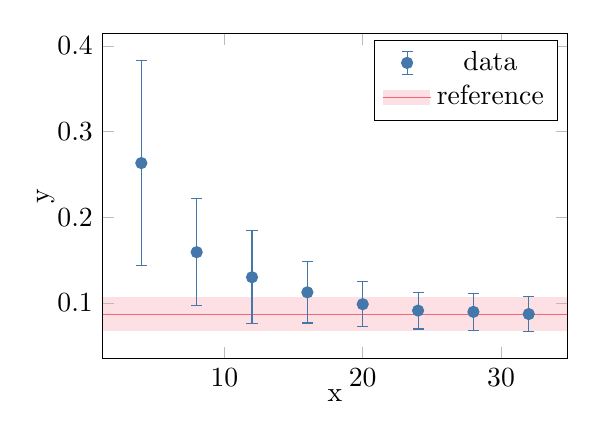
\begin{tikzpicture}
    \begin{axis}[
        width=0.4*\w,
        height=0.28*\w,
        scale only axis=true,
        xlabel = {x},
        ylabel = {y},
        x label style = {yshift=2mm},
        y label style = {yshift=-2mm},
        clip marker paths=true,
        axis on top
        ]

        \fill[T-Q-B5!20] (0,0.1068558) -- (40,0.1068558) -- (40,0.0668558) -- (0,0.0668558) -- cycle;
        \draw[T-Q-B5] (0,0.0868558) -- (40,0.0868558);

        \addplot[color=T-Q-B1, mark=*, only marks, forget plot]
            plot[/pgfplots/error bars/.cd, x dir=none, y dir=both, y explicit,
                error mark=-, error bar style={color=T-Q-B1}]
            coordinates {
                (4,0.263148) +- (0.120064,0.120064)
                (8,0.159158) +- (0.0621894,0.0621894)
                (12,0.129892) +- (0.0543303,0.0543303)
                (16,0.112302) +- (0.0358508,0.0358508)
                (20,0.098435) +- (0.02648,0.02648)
                (24,0.0909784) +- (0.0215048,0.0215048)
                (28,0.0894657) +- (0.0212992,0.0212992)
                (32,0.0869343) +- (0.0202553,0.0202553)
            };
        \addlegendimage{T-Q-B1, mark=*, only marks, error bar legend};
        \addlegendentry{data};
        \addlegendimage{draw=T-Q-B5, fill=T-Q-B5!20, custom area legend};
        \addlegendentry{reference};

    \end{axis}
    \end{tikzpicture}
    \cprotect\caption{This plot breaks rule 3 by using the shade \verb?T-Q-B5!20? for the error band of the reference, but it is still colorblind-safe.}
    \label{fig:errorbar_plot}
\end{figure}

There are additional guidelines that should be kept in mind when typesetting colorblind-safe documents.
Their importance may vary between different applications, so try to follow them as best as possible, at your own judgement.
In no particular order, they are:
\begin{itemize}
    \item \hlc{Do not convey information only through color!}\newline
        When possible, encode the information the color provides also in a different way, e.g., through text, patterns or symbols.
    \item \hlc{Do not use color for information and aesthetics simultaneously!}\newline
        Color is often also used for aesthetic reasons, e.g., on a scientific poster.
        While this is ok in principle, do not mix information and aesthetics within the same visual unit, as this makes it more difficult to extract the encoded information.
    \item \hlc{Do not use rainbow color schemes!}\newline
        Due to the many different colors in a rainbow color scheme, they are very difficult to distinguish for people with color vision deficiencies (even when the scheme is tuned for this purpose).
        Therefore, it is best to avoid them.
        If you insist on using them, Paul Tol provides both a discrete as well as a continuous version, which are optimized to be as distinguishable as possible.
\end{itemize}

\section{Provided color schemes}\label{sec:colors}
The color schemes provided are split into three groups:
\begin{itemize}
    \item Qualitative schemes:\newline
        These schemes are used to convey qualitative information, such as different data sources, countries or manufacturers.
        They should usually be used for coloring text or distinguishing different lines/bars in a plot.
    \item Diverging color schemes:\newline
        When quantitative data ranges between two extremes, and the middle is being considered ``neutral'', a diverging color scheme should be used.
        Examples for this kind of data might be test grades, temperatures or pH values.
    \item Sequential color schemes:\newline
        For quantitative data without an important midpoint, sequential color schemes should be preferred over diverging ones.
        This is especially true for quantites that start from $0$.
        They can be used to denote for example velocities, concentrations or pressures.
\end{itemize}

For each type of schemes, this package provides a range of options.
\Cref{sec:Tol_schemes} shows the schemes designed by Paul Tol~\cite{Tol}, which include qualitative, diverging and sequential schemes (see \cref{sec:T-Q,sec:T-D,sec:T-S}).
In \cref{sec:OkabeIto}, the Okabe Ito color scheme~\cite{Ichihara_2008} is provided, which is probably the most famous qualitative colorblind-safe color scheme due to it being mentioned in various articles in high-ranking journals.

All of the schemes are colorblind-safe, and some are optimized for printout or designed for a particular purpose.
This is denoted under the scheme name.\clearpage

\subsection{Paul Tol's color schemes}\label{sec:Tol_schemes}

\subsubsection{Qualitative color schemes}\label{sec:T-Q}
\begin{minipage}{0.5\textwidth}
    \centering
    \scalebox{0.7}{\drawScheme{T-Q-B}}\\
    \textbf{B}right\\
    \phantom{pb}
\end{minipage}\hfill%
\begin{minipage}{0.5\textwidth}
    \centering
    \scalebox{0.7}{\drawScheme{T-Q-V}}\\
    \textbf{V}ibrant
\end{minipage}

\begin{minipage}{0.5\textwidth}
    \centering
    \scalebox{0.7}{\drawScheme{T-Q-HC}}\\
    \textbf{H}igh-\textbf{C}ontrast\\
    works for black and white printout
\end{minipage}\hfill%
\begin{minipage}{0.5\textwidth}
    \centering
    \scalebox{0.7}{\drawScheme{T-Q-MC}}\\
    \textbf{M}edium-\textbf{C}ontrast\\
    works for black and white printout
\end{minipage}

\begin{center}
    \scalebox{0.7}{\drawScheme{T-Q-M}}\\
    \textbf{M}uted
\end{center}

\begin{minipage}{0.5\textwidth}
    \centering
    \scalebox{0.7}{\drawScheme{T-Q-PH}}\\
    \textbf{P}ale \textbf{H}ighlight\\
    specifically for text background
\end{minipage}\hfill%
\begin{minipage}{0.5\textwidth}
    \centering
    \scalebox{0.7}{\drawScheme{T-Q-DT}}\\
    \textbf{D}ark \textbf{T}ext\\
    specifically for text color
\end{minipage}

\begin{center}
    \scalebox{0.7}{\drawScheme{T-Q-L}}\\
    \textbf{L}ight\\
    less distinguishable than other schemes,\\ mostly meant for filling in labelled cells
\end{center}\clearpage

\subsubsection{Diverging color schemes}\label{sec:T-D}
For diverging schemes, when a continuous scheme is needed, the colors are allowed to be linearly interpolated.
When using the option \verb!pgf!, the interpolations are available as colormaps with the names of their color scheme.

\begin{center}
    \scalebox{0.7}{\drawScheme{T-D-S}}\\
    \drawSchemeC[0.6\textwidth]{T-D-S}\\
    \textbf{S}unset
\end{center}

\begin{center}
    \scalebox{0.7}{\drawScheme{T-D-N}}\\
    \drawSchemeC[0.9\textwidth]{T-D-N}\\
    \textbf{N}ightfall
\end{center}

\begin{center}
    \scalebox{0.7}{\drawScheme{T-D-BR}}\\
    \drawSchemeC[0.5\textwidth]{T-D-BR}\\
    \textbf{B}u\textbf{R}d
\end{center}

\begin{center}
    \scalebox{0.7}{\drawScheme{T-D-PG}}\\
    \drawSchemeC[0.5\textwidth]{T-D-PG}\\
    \textbf{P}R\textbf{G}n
\end{center}\clearpage

\subsubsection{Sequential color schemes}\label{sec:T-S}
For most sequential schemes, a continuous scheme can be obtained again by linearly interpolating the colors.
The only exception to this is the \emph{discrete rainbow} scheme, which has an explicitly continuos variation, the \emph{smooth rainbow} scheme.
When using the option \verb!pgf!, the interpolations are available as colormaps with the names of their color scheme.

When the discrete scheme is not shown, this is because there are too many colors in it.

\begin{center}
    \scalebox{0.7}{\drawScheme{T-S-YOB}}\\
    \drawSchemeC[0.5\textwidth]{T-S-YOB}\\
    \textbf{Y}l\textbf{O}r\textbf{B}r
\end{center}

\begin{center}
    \drawSchemeC[0.9\textwidth]{T-S-IR}\\
    \textbf{Ir}idescent
\end{center}

\begin{center}
    \scalebox{0.7}{\drawScheme{T-S-IN}}\\
    \drawSchemeC[0.6\textwidth]{T-S-IN}\\
    \textbf{In}candescent\\
    not print-friendly
\end{center}

\begin{center}
    \scalebox{0.7}{\drawScheme{T-S-DR}}\\
    \textbf{D}iscrete \textbf{R}ainbow\\
    Do not interpolate!
\end{center}

\begin{center}
    \drawSchemeC[\textwidth]{T-S-SR}\\
    \textbf{S}mooth \textbf{R}ainbow\\
\end{center}\clearpage

\subsection{Okabe Ito qualitative color scheme}\label{sec:OkabeIto}
This is the qualitative color scheme commonly known as the \emph{Okabe Ito} color palette~\cite{Ichihara_2008}.

\begin{center}
    \scalebox{0.7}{\drawScheme{OI}}\\
    \textbf{O}kabe \textbf{I}to
\end{center}

\section{Provided commands}
\cprotect\marg{\verb!\drawScheme{...}!}%
The discrete visualizations of color schemes given in this documentation are created with the command \verb!\drawScheme{...}!.
The name of the color scheme should be provided to the command, e.g.\ \verb!\drawScheme{T-Q-B}! to print the \emph{qualitative bright} scheme by Tol.
Note that this command is not available when the package option \verb!no-tikz! is used.

\cprotect\marg{\verb!\drawSchemeC{...}!}%
The continuous visualizations of color schemes given in this documentation are created with the command \verb!\drawSchemeC{...}!.
The name of the color scheme should be provided to the command, e.g.\ \verb!\drawSchemeC{T-D-S}! to print the \emph{diverging sunset} scheme by Tol.
Note that this command only works for color schemes that are allowed to be interpolated, and that the command is only available when the package option \verb!pgf! is used.

\clearpage
\printbibliography

\end{document}
